% Preamble
\documentclass[twocolumn]{article}

% Packages
\usepackage[T1]{fontenc} % Used
\usepackage[utf8]{inputenc} % Used
\usepackage{indentfirst} % Used
\usepackage{lipsum} % Used
\usepackage{amsmath} % Used
\usepackage[margin=1in]{geometry}  % Used
\usepackage[font=small,labelfont=bf]{caption} % Used
\usepackage{hyperref} % Used
\usepackage{fancyhdr} % Used
\usepackage{tikz} % Used
\usetikzlibrary{graphs} % Used
\usetikzlibrary{chains} % Used
\usetikzlibrary{positioning} % Used
\usetikzlibrary{quotes} % Used

\usepackage{subcaption}
\usepackage{newfloat}

\usepackage{booktabs} % Used
\usepackage{tikz-network} % Used

\usepackage{multirow}
\usepackage{graphicx}

\pagestyle{fancy}

\fancyhead{}
\lhead{
    
\includegraphics[scale=0.13]{images/logo.png}
}
\rhead{
    Distributed and Parallel Computing \\
    2019/2020
    \footnotesize
}

\fancyfoot[C]{\thepage}

\date{}

\title{
    
\includegraphics[scale=0.2]{images/logo.png}\\
    \vskip 0.5em
    \Huge Distributed and Parallel Computing\\
    \LARGE OpenMPI Report\\
}

\author{
    Pedro Rio\\
    \textit{MSc Data Science and Engineering}\\
    \textit{Instituto Superior Técnico}\\
    \textit{97241}
    \and
    Sebastião Maia Serqueira\\
    \textit{MSc Data Science and Engineering}\\
    \textit{Instituto Superior Técnico}\\
    \textit{97108}\\
    \and
    Eduardo Machado\\
    \textit{MSc Data Science and Engineering}\\
    \textit{Instituto Superior Técnico}\\
    \textit{97133}
}

% Document
\begin{document}
    \maketitle

    \section{Program Overview}\label{sec:program-overview}
    The program serial implementation is divided into four main parts:

    \subsection{ReadInput}\label{subsec:readinput}
    A for loop is used to read each line of the instance file and get the number of iterations, users, items, latent features, non zero elements and the value of the convergence coefficient.
    After this step, the matrix A and a vector of the indexes of the non zero elements are then populated.

    \subsection{InitialLR}\label{subsec:initiallr}
    The routine provided was used to initialise the matrices L and R.

    \subsection{UpdateLR}\label{subsec:updatelr}
    A recommendation score is predicted for each one of the non zero elements of matrix A, using its i and j indexes to compute the internal product of the row i of the matrix L and the column j of matrix R\@.
    Afterwards, the differential between the real value of the non zero element in matrix A and its prediction is computed for all the non zero elements.
    Finally and also for each one of the non zero elements of matrix A, the selected column of matrix L and a row of R are updated to decrease the obtained differential as a function of the existing differential, the convergence coefficient and the stored matrices L and R\@.
    The function is repeated in a loop for the number of iterations and for each iteration the program stores the values of the matrices L and R and uses them to update the matrices L and R\@.

    \subsection{FilterFinalMatrix}\label{subsec:filterfinalmatrix2}
    The matrix B is computed as the multiplication of matrices L and R. Afterwards, for each row of matrix B, the maximum value is computed without taking into account the the non zero elements.
    The location of the values are stored in a vector and streamed to the standard output.

    \section{OpenMP Version}\label{sec:openmp-version}

    \subsection{Foster Methodology}
    \label{subsec:foster-methodology}
    \subsubsection{ReadInput}
    \textbf{Partitioning}

    \textbf{Communication}

    \textbf{Agglomeration and Mapping}

    \subsubsection{InitialLR}
    \textbf{Partitioning}

    \textbf{Communication}

    \textbf{Agglomeration and Mapping}

    \subsubsection{UpdateLR}
    \textbf{Partitioning}

    \textbf{Communication}

    \textbf{Agglomeration and Mapping}

    \subsubsection{FilterFinalMatrix}
    \textbf{Partitioning}

    \textbf{Communication}

    \textbf{Agglomeration and Mapping}


    \subsection{Decompositions}
    \label{subsec:decompostions}
    In our openMP implementation we used the Functional and Data parallelism decompositions in the following way:

    \textbf{Data Parallelism} - was firstly used to read the input files and to perfom the calculations of an initial predicted value of B ($L$ x $R$), the delta coefficient, updating the previous $L$ and $R$ matrices and in the calculation of the final matrix B\@.

    \subsection{Synchronization}
    \label{subsec:synchronization}
    In our implementation we were not faced with the necessity of explicitly using synchronization controls, since our code is divided into 4 main blocks, meaning that the synchronization happens implicitly after each block is run.
    Also, we note that synchronization happens after each block of code has finished.


    \section{Optimisations} \label{sec:optimisations}

    In order to optimise the program we parallelized all the blocks except initialLR. The function cannot be parallelized because it incorporates a random function that must be called sequentially.
    If the function was parallelized , the results would be wrong due to data races among the threads.
    Regarding the other blocks:

    \subsection{ReadInput}\label{subsec:readinput2}
    The first parallelization zone in the program happens in the read input function.
    This function, as the name describes, will read the lines of the file and save it on variables.
    First, we save the lines through a 'for' to a vector since it is not possible to parallelise.
    Then, we read the first 4 lines to save number of Iterations, convergence coefficient, number of features and others.
    Lastly, we have to read the rest of the lines depending in each file.
    In order to do that, we parallelized the for cycle by using the schedule 'guided' to optimize the parallelization.
    In guided schedule, is assigned to each thread a block of decreasing size.
    The size of each block is proportional to the number of unassigned iterations divided by the number of threads, decreasing to chunk.

    \subsection{UpdateLR}\label{subsec:updatelr2}
    The block updateLR is also parallelized.
    All the function updateLR is parallelized because we had three mini fuctions inside updateLR and these are composed by cycles for's.
    Obviously all these are parallelized.
    The first mini function has a "pragma omp for collapse(2)", which means that two cycles for are transformed into one and this one is parallelized with a schedule guided.
    The second mini fuction has a cycle for parallelized with schedule guided.
    The last one also has a "pragma omp for collapse(2)" for the same reason.
    We decided to use guided schedule on the first and third mini function because it exists some iteration that are bigger than others.
    Due to these iterations guided schedule improve the parallelization.

    \subsection{FilterFinalMatrix}\label{subsec:filterfinalmatrix}
    The other zone that is parallelized is the 'filterFinalMatrix' function.
    This function consists in 'computeB' function and in three for cycles which are parallelized.
    As the name describes the computeB function will calculate B for each matrix position.
    Inside this function exists a triple loop which we parallelized with a '\#pragma omp for collapse(3)'.
    The three for cycles that belong to the 'filterFinalMatrix' function are individually parallelized.
    Two of them are settled with schedule guided.
    The last one is settled with ordered.
    It needs this setting because the cycle for is printing on the console and it needs to print in the correct order.

    \section{Evaluation}\label{sec:evaluation}

    \begin{figure}[h]
        \caption{Speedup}
%        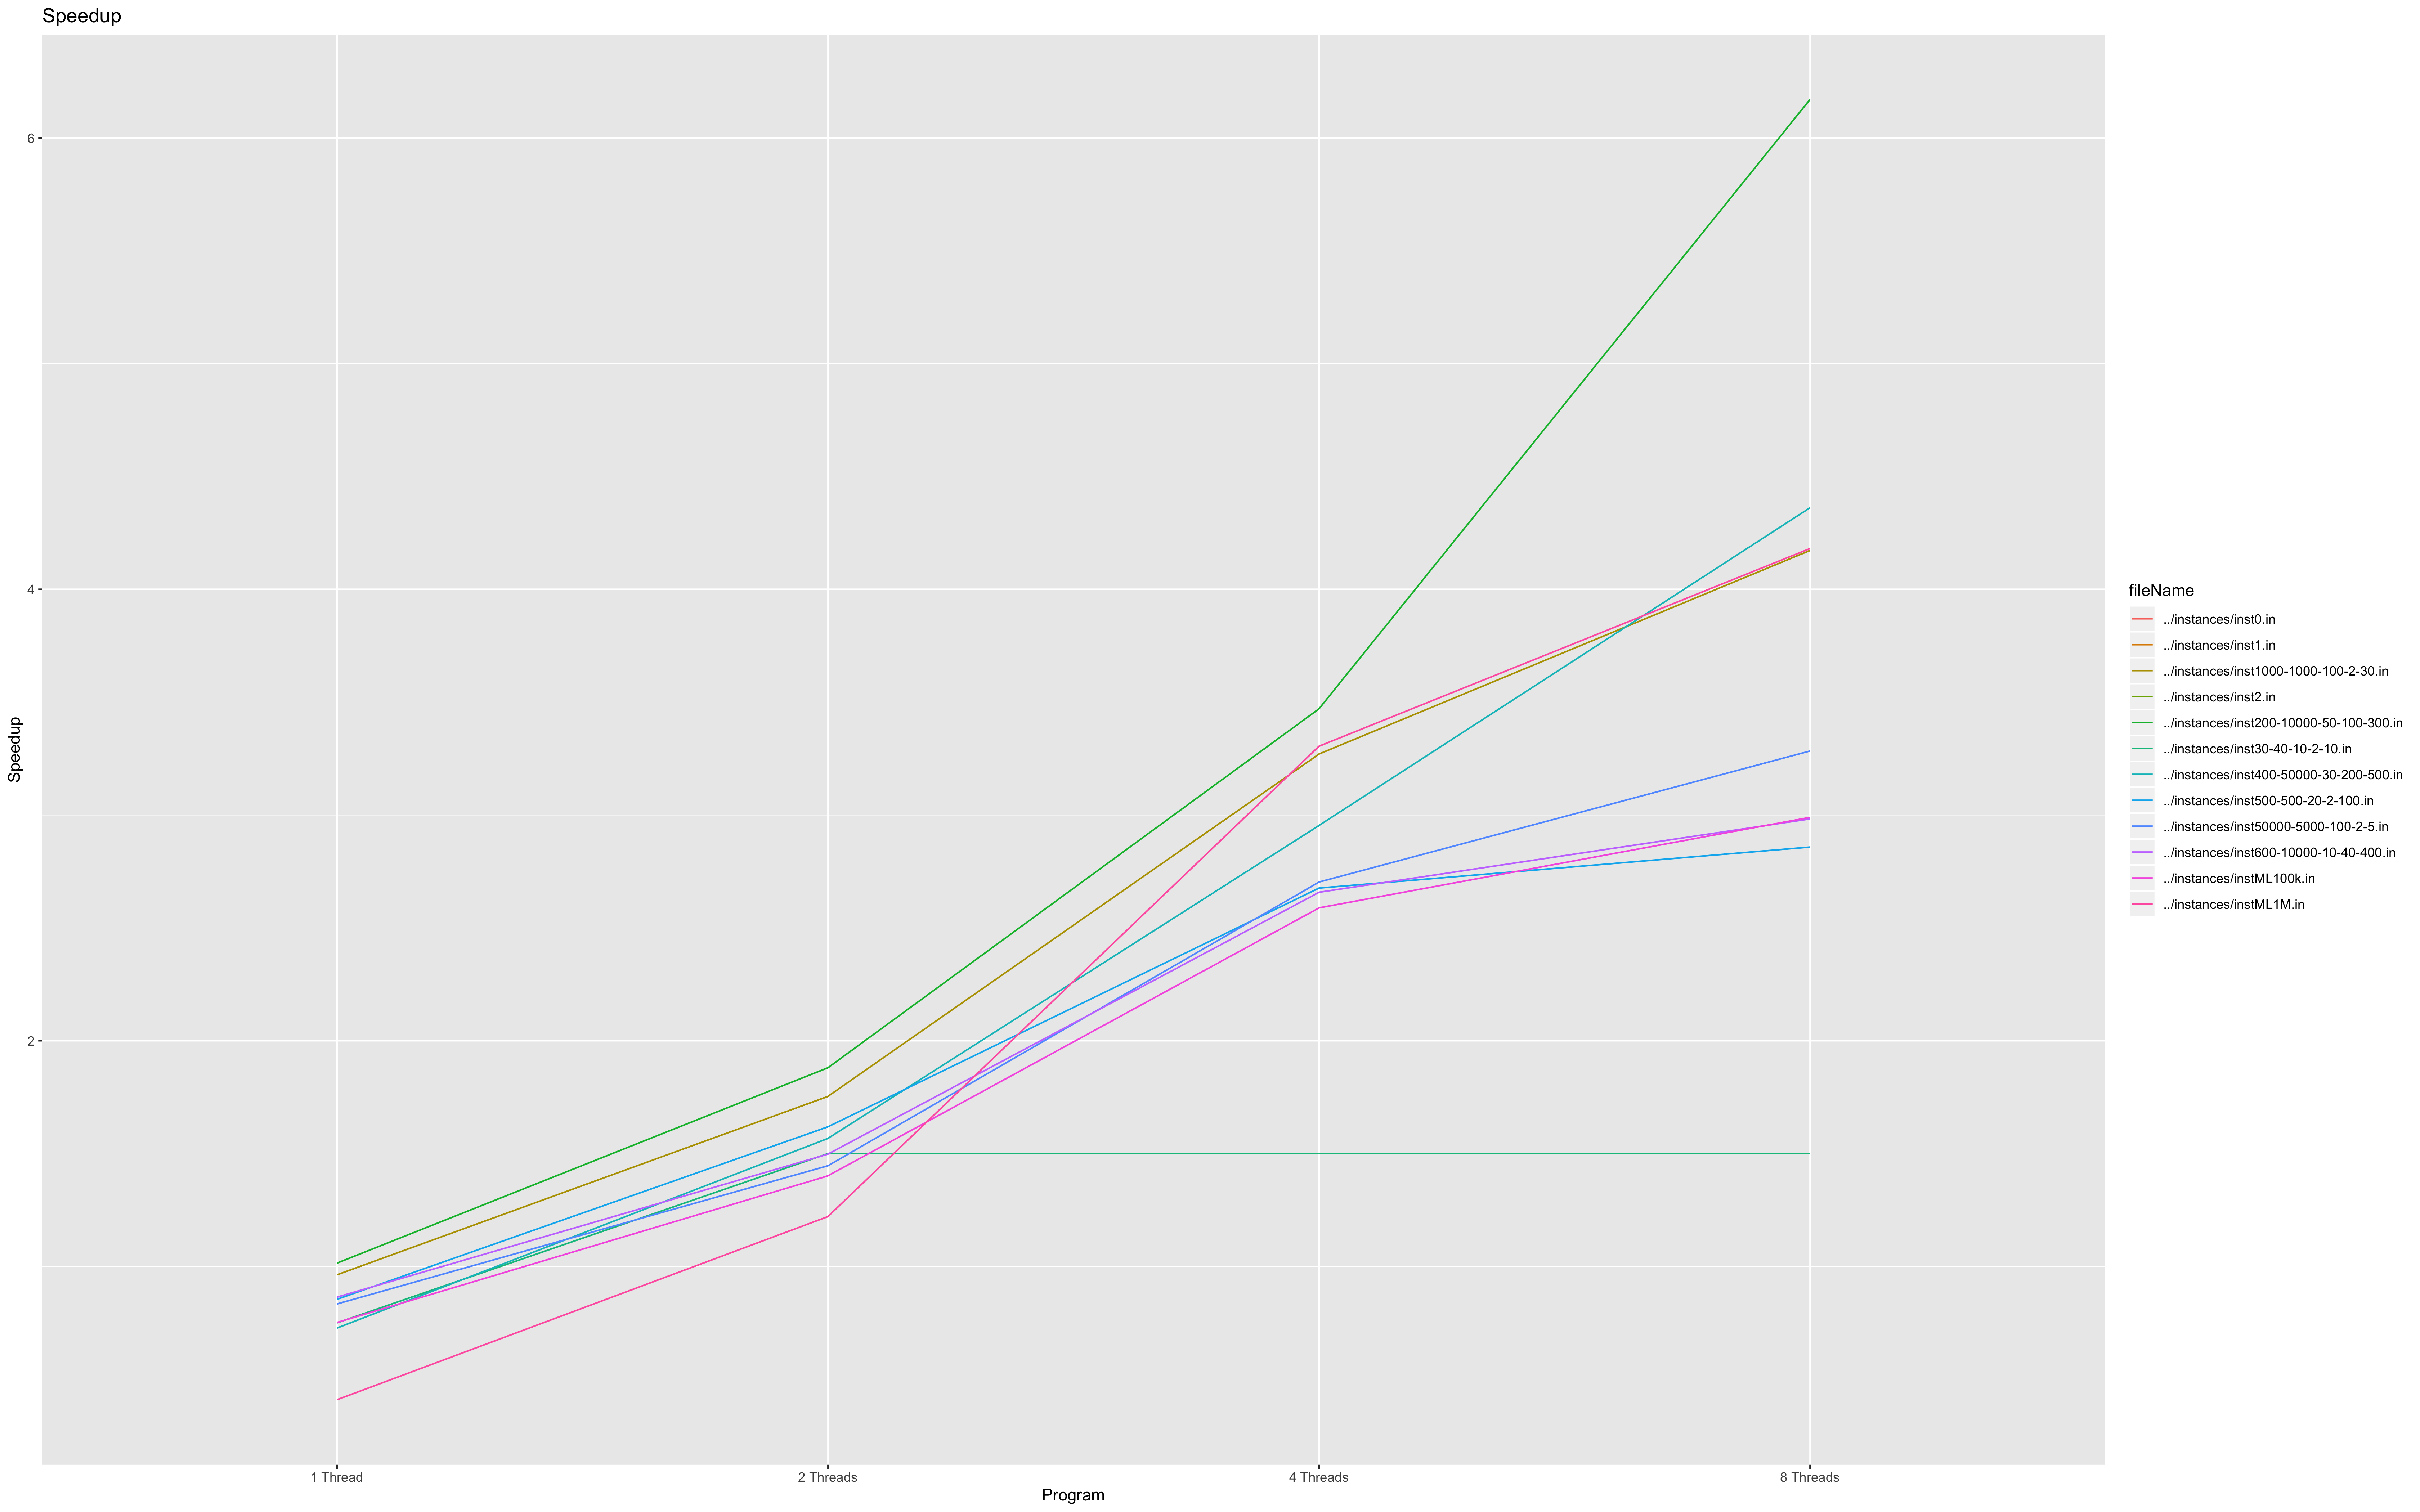
\includegraphics[width=1\linewidth]{speedup.png}
        \label{fig:Ng2}
    \end{figure}

    \begin{table}[!h]
        \caption{\label{tab:speedup}Speedup}
        \centering
        \resizebox{\linewidth}{!}{
            \begin{tabular}[t]{lrrrr}
                \toprule
                fileName & 1 Thread & 2 Threads & 4 Threads & 8 Threads\\
                \midrule
                inst0.in & NaN & NaN & NaN & NaN\\
                inst1.in & NaN & NaN & NaN & NaN\\
                inst1000-1000-100-2-30.in & 0.9628647 & 1.753623 & 3.270270 & 4.172414\\
                inst2.in & NaN & NaN & NaN & NaN\\
                inst200-10000-50-100-300.in & 1.0146163 & 1.880361 & 3.470833 & 6.170370\\
                \addlinespace
                inst30-40-10-2-10.in & 0.7500000 & 1.500000 & 1.500000 & 1.500000\\
                inst400-50000-30-200-500.in & 0.7269504 & 1.567278 & 2.953890 & 4.361702\\
                inst500-500-20-2-100.in & 0.8542435 & 1.618881 & 2.676301 & 2.858025\\
                inst50000-5000-100-2-5.in & 0.8337190 & 1.446101 & 2.703108 & 3.283854\\
                inst600-10000-10-40-400.in & 0.8638906 & 1.497845 & 2.657744 & 2.982833\\
                \addlinespace
                instML100k.in & 0.7516242 & 1.401677 & 2.588640 & 2.990060\\
                instML1M.in & 0.4093360 & 1.221217 & 3.304762 & 4.180723\\
                \bottomrule
            \end{tabular}}
    \end{table}

    In our opinion, our OpenMP implementation improves the speedup when it has more threads working as supposed.
    Nevertheless, we know by Amdahl's law that the speed is limited by the total time needed for the execution of the sequential part.
    As our program is not completely parallelized, the speedup cannot increase linearly with the amount of threads.

    \begin{figure}[h]
        \caption{Total Execution Time}
%        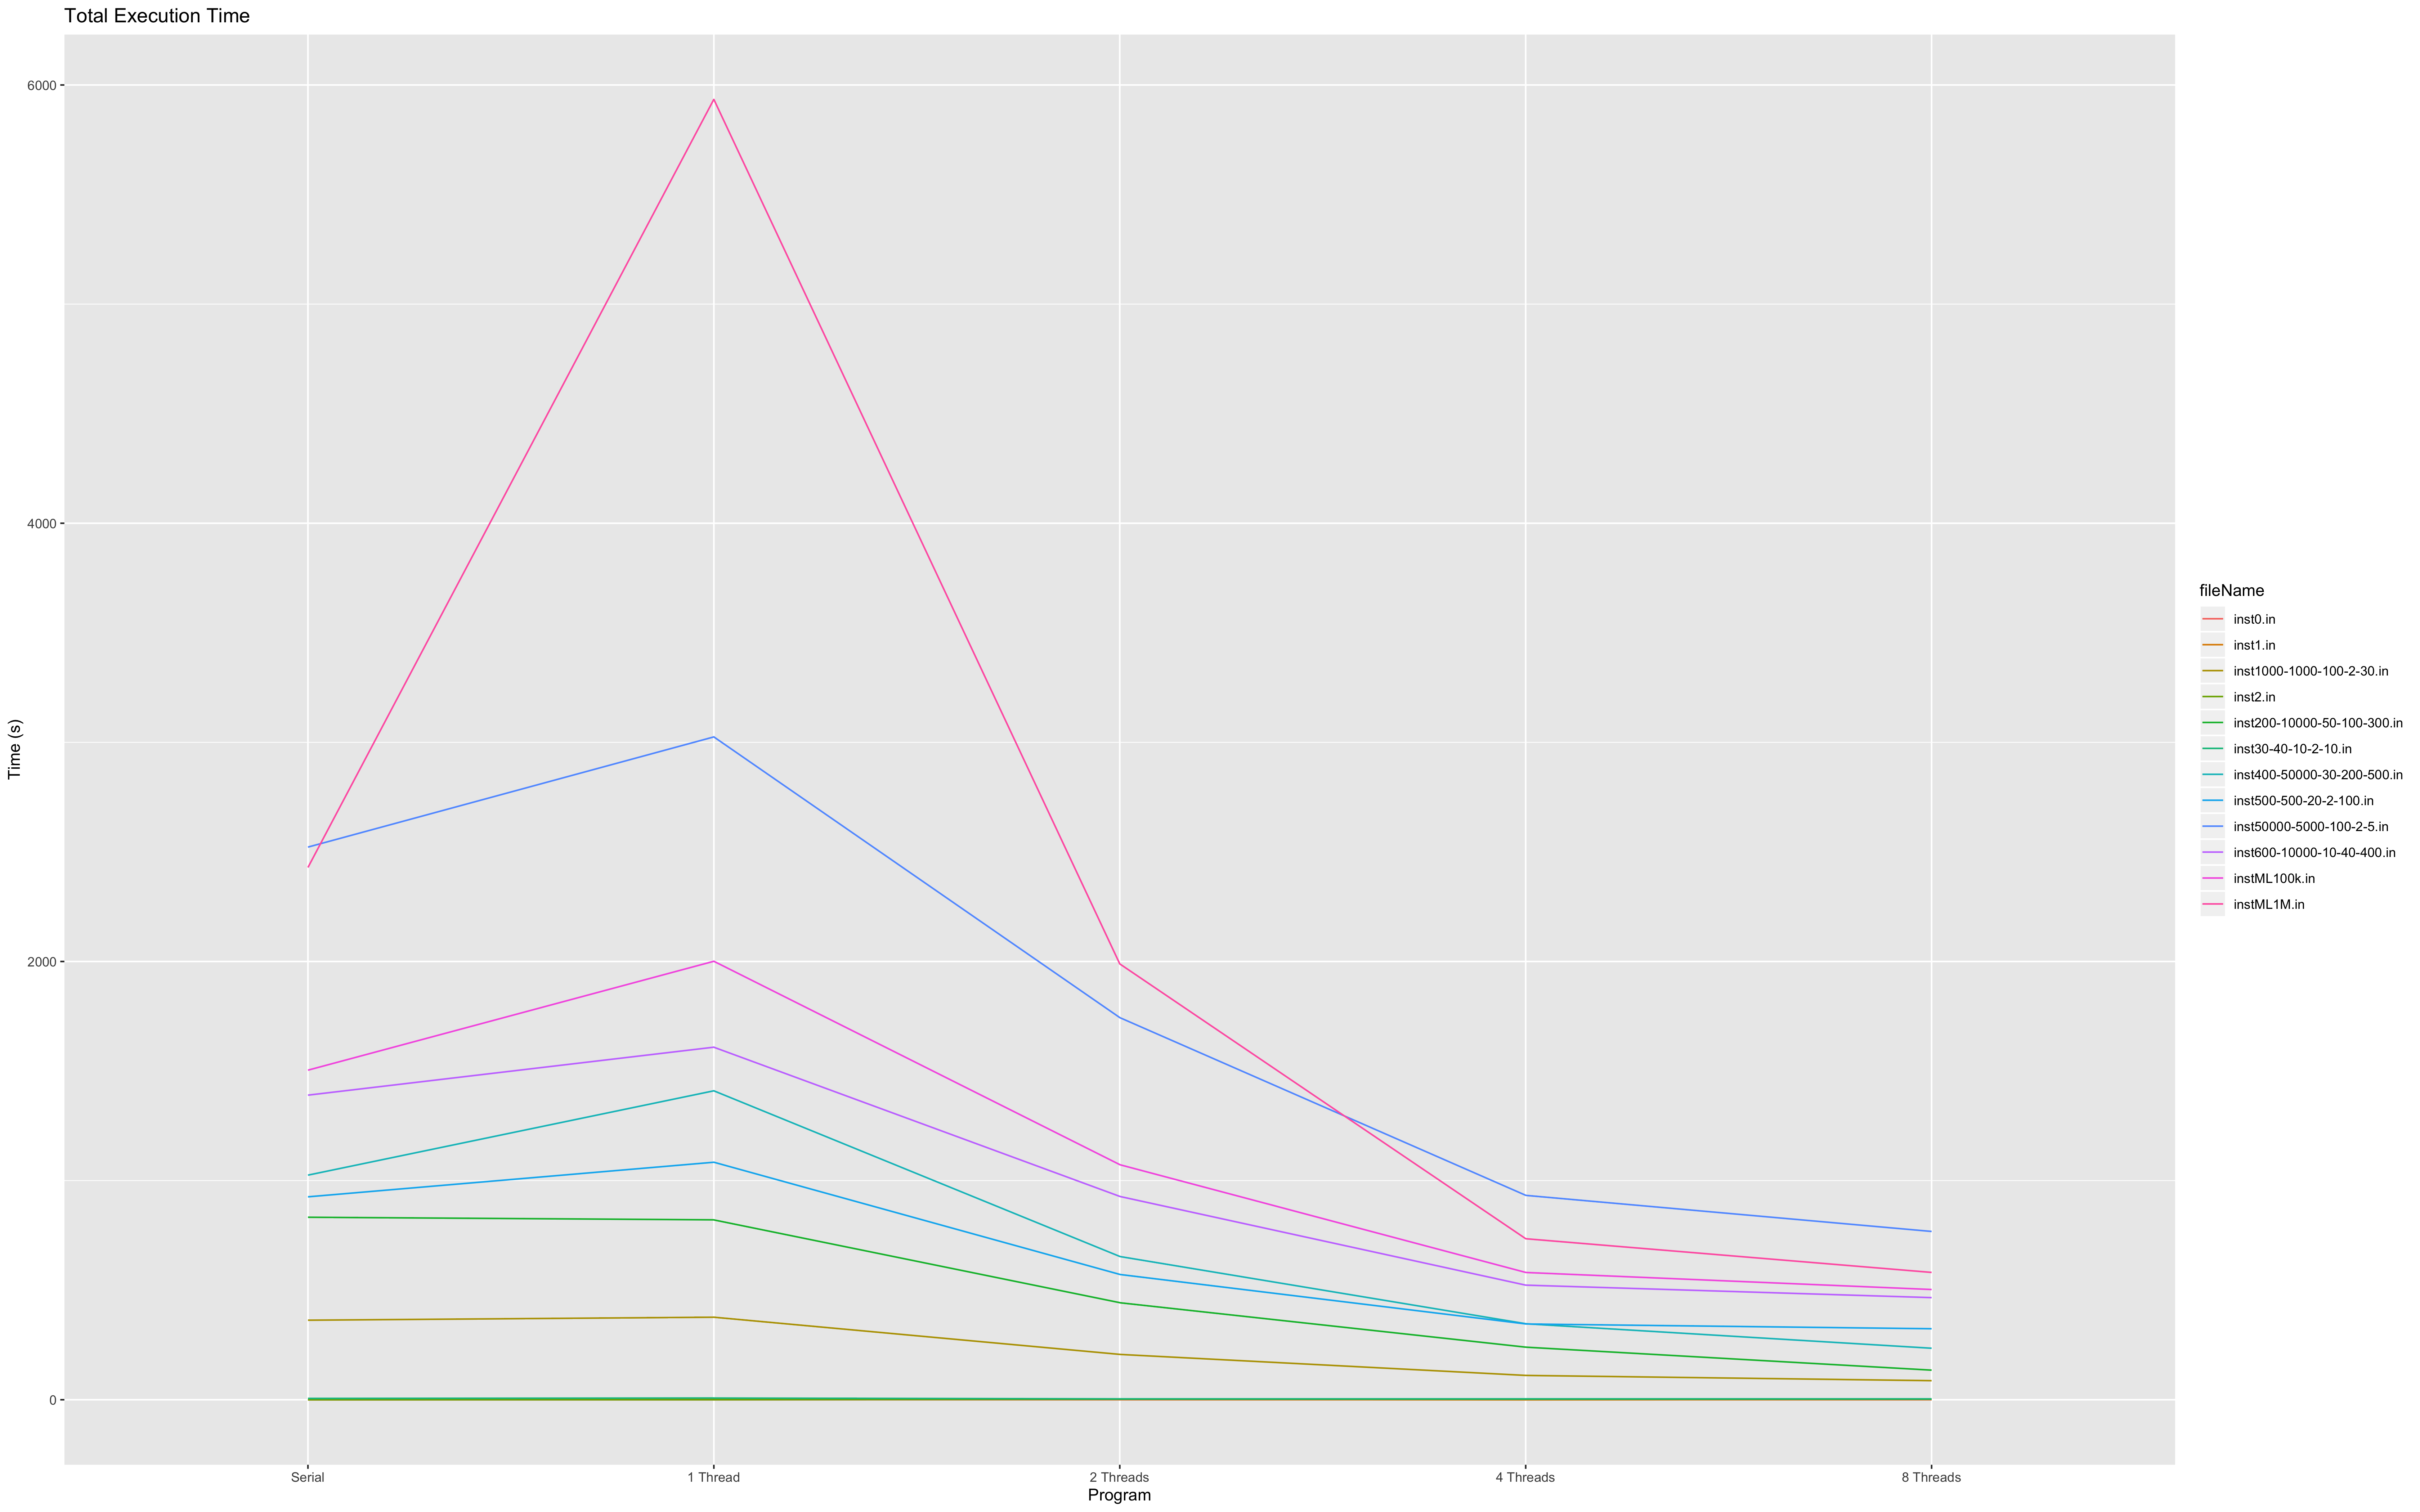
\includegraphics[width=1\linewidth]{time.png}
        \label{fig:Ng1}
    \end{figure}

    \begin{table}[!h]
        \caption{\label{tab:time}Total Execution Time}
        \centering
        \resizebox{\linewidth}{!}{
            \begin{tabular}[t]{lrrrr}
                \toprule
                fileName & 1 Thread & 2 Threads & 4 Threads & 8 Threads\\
                \midrule
                inst0.in & 0 & 0 & 0 & 0\\
                inst1.in & 2 & 2 & 0 & 2\\
                inst1000-1000-100-2-30.in & 377 & 207 & 111 & 87\\
                inst2.in & 0 & 2 & 2 & 2\\
                inst200-10000-50-100-300.in & 821 & 443 & 240 & 135\\
                \addlinespace
                inst30-40-10-2-10.in & 8 & 4 & 4 & 4\\
                inst400-50000-30-200-500.in & 1410 & 654 & 347 & 235\\
                inst500-500-20-2-100.in & 1084 & 572 & 346 & 324\\
                inst50000-5000-100-2-5.in & 3025 & 1744 & 933 & 768\\
                inst600-10000-10-40-400.in & 1609 & 928 & 523 & 466\\
                \addlinespace
                instML100k.in & 2001 & 1073 & 581 & 503\\
                instML1M.in & 5934 & 1989 & 735 & 581\\
                \bottomrule
            \end{tabular}}
    \end{table}
%
%    \cleardoublepage~\nocite{*}
%    \bibliography{main}
%    \bibliographystyle{unsrt}
\end{document}
